\documentclass[10pt,a4paper]{article}
\usepackage[utf8]{inputenc}
\usepackage{ucs}
\usepackage{amsmath}
\usepackage{amsfonts}
\usepackage{amssymb}
\usepackage{graphicx}


\begin{document}
\title{Segunda semana de trabajo [07 - 11 de abril]}
\author{Milton Inostroza Aguilera}
\date{13 Abril de 2008}
\clearpage
\maketitle

\begin{abstract}
Para un manejo eficiente en la inspección de los scripts objetivo, se hace indispensable estudiar el bytecode de Python.  El inspector construído funciona de manera correcta y eficiente pero tiene problemas de diseño.\\

Por lo anterior se reconstruirá completamente con una fuerte orientación a objetos.
\end{abstract}
\pagebreak
\section{Desarrollo}
La semana comenzó por configurar un servidor local svn para poder manejar de mejor forma los cambios de versiones de los scripts programados.\\

Como tarea principal se tiene que se debe enviar un mensaje a la base de datos de TOD cuando ocurran los siguentes eventos:
\begin{itemize}
\item call/return
\item set local/attribute
\item registration
	\begin{itemize}
	\item new class
	\item new local
	\item new attribute
	\item new method / function
	\end{itemize} 
\end{itemize}

Examinando de mejor forma la función settrace se ha decidido eliminar el método \_\_getattribute\_\_ del descriptor, ya que settrace captura la llamada de métodos.\\

Para entender de mejor forma lo que se debe hacer ponemos un ejemplo:
\begin{verbatim}
def foo():
    x = 1
    a = x
    x = 20
\end{verbatim}

Lo que debe generar los siguientes mensajes, de forma aproximada:
\begin{verbatim}
registration "foo", id = 26, class = None, {'x':1,'a':2}
call #26, target None,..
set #1, valor = 1
set #2, valor = 1
set #1, valor = 20
return
\end{verbatim}

Se modifica la estructura de register\_locals para poder asignar un id a los objetos de primer nivel (clase, metodo y funcion).  La estructura queda de la siguiente manera:

\begin{verbatim}
register_locals = {'code':(id,{'key':value,'key2':value2})}
\end{verbatim}

Al momento de instanciar una clase el objeto igual debe llevar un identificador único, esto lo hacemos al momento que se invoca al método \_\_init\_\_ de la clase.  De la siguiente manera modificamos al objeto:

\begin{verbatim}
id = Id.__get__()
obj.__dict__.update({'_pytod_id':id})
\end{verbatim}

Al haber terminado de realizar todas las modificaciones que se necesitaban, nos hemos dado cuenta que la forma de capturar la huella del script objetivo es ineficiente y por lo tanto es impresentable.  El problema radica en que capturamos el diccionario global locals para poder acceder a las variables locales que se estan modificando, pero por cada línea que ejecutamos locals siempre nos devuelve todas las variables locales del frame y por lo tanto enviamos a la base de datos eventos set's repetidos, lo que por una parte es ineficiente pero por otra y la más importante es que se pierde el control de saber el momento exacto la variable x cambio a un valor y.\\

Se toma la decision de comenzar a inspeccionar el bytecode Python para ver en el momento que se modifican las variables locales y asi poder enviar un evento set que corresponda exactamente al cambio de valor de la variable.\\

A priori las instrucciones que nos interesan son LOAD\_CONST y STORE\_NAME \cite{bytecode}, y el módulo que debemos estudiar para realizar las inspecciones al bytecode en tiempo de ejecución es inspect.

Se crea una estructura llamada lnotab para almacenar la línea de código con su correspondiente indice de bytes en el bytecode, ejemplo:

\begin{verbatim}
lnotab = {'11':(6,12),'12':(12,21),'15':(21,30),'17':(30,41)}
\end{verbatim}

Esto significa que para la línea 11 del código fuente los indices a ejecutar del bytecode son desde 6 hasta 12.

\section{bytecode}

TOS

	Top of the Stack.\\\\
TOS1

	Top\_most stack item.\\\\
LOAD\_CONST \textit{consti}

	pushes "co\_consts[\textit{consti}]" onto the stack. \\\\
STORE\_FAST \textit{var\_num}

	stores TOS into the local "co\_varnames[\textit{var\_num}]" onto the stack.\\\\
RETURN\_VALUE

	returns with TOS to the caller of the function.\\\\
LOAD\_FAST \textit{var\_num}

	pushes a reference to the call co\_varnames[\textit{var\_num}] onto the stack.\\\\
STORE\_ATTR \textit{namei}

	implements TOS.name = TOS1, where \textit{namei} is the index of name in code.co\_names.\\\\
MAKE\_FUNCTION \textit{argc}

    Pushes a new function object on the stack. TOS is the code associated with the function. The function object is defined to have argc default parameters, which are found below TOS.\\\\
LOAD\_LOCALS

    Pushes a reference to the locals of the current scope on the stack. This is used in the code for a class definition: After the class body is evaluated, the locals are passed to the class definition.\\\\

Para la siguiente funcion:
\begin{verbatim}
def myfunc():
    a = 2
    b = 3
\end{verbatim}

Se tiene el siguiente bytecode:

\begin{verbatim}
 48           0 LOAD_CONST               1 (2)
              3 STORE_FAST               0 (a)

 49           6 LOAD_CONST               2 (3)
              9 STORE_FAST               1 (b)
             12 LOAD_CONST               0 (None)
             15 RETURN_VALUE 
\end{verbatim}

El lnotab correspondiente sería:

\begin{verbatim}
lnotab = {'49':(6,15),'48':(0,3)}
\end{verbatim}

Existe un detalle importante en la impresión del bytecode y es que los bytes 12 y 15 son instrucciones propias de return que aparecen en la linea 49 que es en la cual se modifica una variable local.  Probamos el siguiente código:

\begin{verbatim}
def myfunc():
    a = 2
    b = 3
	return
\end{verbatim}

Se tiene el siguiente bytecode:

\begin{verbatim}
 48           0 LOAD_CONST               1 (2)
              3 STORE_FAST               0 (a)

 49           6 LOAD_CONST               2 (3)
              9 STORE_FAST               1 (b)

 50          12 LOAD_CONST               0 (None)
             15 RETURN_VALUE 
\end{verbatim}

Por lo que podemos deducir que Python si el programador no escribe la instrucción return implicitamente el la añade.

Analizando algunas estructuras internas de code vemos que:

\begin{verbatim}
code.co_consts = (NONE, 2, 3)
code.co_varnames = ('a', 'b')
\end{verbatim}

Si agregamos un argumento a la función y no lo usamos, este no aparece en el bytecode pero si aparece en code.co\_varnames, code.co\_consts no se ve afectado, code.co\_argcount = 1, code.co\_nlocals = 3. \\

En todos los casos anteriores siempre code.co\_names esta vacío.\\

Es interesante examinar el siguiente caso:

\begin{verbatim}
class myclass():

    def __init__(self):
        self.a = 10
        x = 8
        return

    def mymethod(self, q):
        self.b = q
        return
\end{verbatim}

Al momento de terminar de definir la clase, el bytecode asociado es:

\begin{verbatim}
 42           0 LOAD_NAME                0 (__name__)
              3 STORE_NAME               1 (__module__)

 43           6 LOAD_CONST               0 (<code object __init__ at 0xb7dae4a0, 
                                            file "ejemplo.py", line 43>)
              9 MAKE_FUNCTION            0
             12 STORE_NAME               2 (__init__)

 48          15 LOAD_CONST               1 (<code object mymethod at 0xb7dae698, 
                                            file "ejemplo.py", line 48>)
             18 MAKE_FUNCTION            0
             21 STORE_NAME               3 (mymethod)
             24 LOAD_LOCALS         
             25 RETURN_VALUE 

\end{verbatim}

Lo que hace en el índice 15 es cargar una referencia de locals en el ambiente actual sobre el stack.  Información sobre algunas estructuras internas de code:

\begin{verbatim}
code.co_argcount = 0
code.co_consts = (<code object __init__ at 0xb7dae4a0, file "ejemplo.py", line 43>,
                  <code object mymethod at 0xb7dae698, file "ejemplo.py", line 48>)
code.co_names = ('__name__', '__module__', '__init__', 'mymethod')
code.co_varnames = ()
code.co_freevars = ()
code.co_cellvars = ()
\end{verbatim}

El bytecode asociado a la llamada del metodo \_\_init\_\_ es:

\begin{verbatim}
 37           0 LOAD_CONST               1 (10)
              3 LOAD_FAST                0 (self)
              6 STORE_ATTR               0 (a)

 38           9 LOAD_CONST               2 (8)
             12 STORE_FAST               1 (x)

 39          15 LOAD_CONST               0 (None)
             18 RETURN_VALUE        

\end{verbatim}

Información sobre algunas estructuras internas de code:

\begin{verbatim}
code.co_argcount = 1
code.co_consts = (None, 10, 8)
code.co_names = ('a',)
code.co_varnames = ('self', 'x')
code.co_freevars = ()
code.co_cellvars = ()
\end{verbatim}

El bytecode asociado a la llamada del metodo mymethod es:

\begin{verbatim}
 49           0 LOAD_FAST                1 (q)
              3 LOAD_FAST                0 (self)
              6 STORE_ATTR               0 (b)

 50           9 LOAD_CONST               0 (None)
             12 RETURN_VALUE 
\end{verbatim}

Información sobre algunas estructuras internas de code:

\begin{verbatim}
code.co_argcount = 2
code.co_consts = (None,)
code.co_names = ('b',)
code.co_varnames = ('self', 'q')
code.co_freevars = ()
code.co_cellvars = ()
\end{verbatim}


Se debe diseñar la funcion getpartcode para extraer las variables que estan siendo modificadas en cierta parte del código.

Por asunto de eficiencia lnotab cambia el contenido de la estructura por:

\begin{verbatim}
lnotab = {next_index:(previous_index,next_index-1)}
\end{verbatim}

Ahora que el script esta estable, se debe rediseñar para dejarlo orientado a objetos, ya que hasta el momento tiene un enfoque procedural.

\pagebreak

El diseño que se ha conceptualizado es el siguiente:

\begin{figure}[hpb]
	\centering
	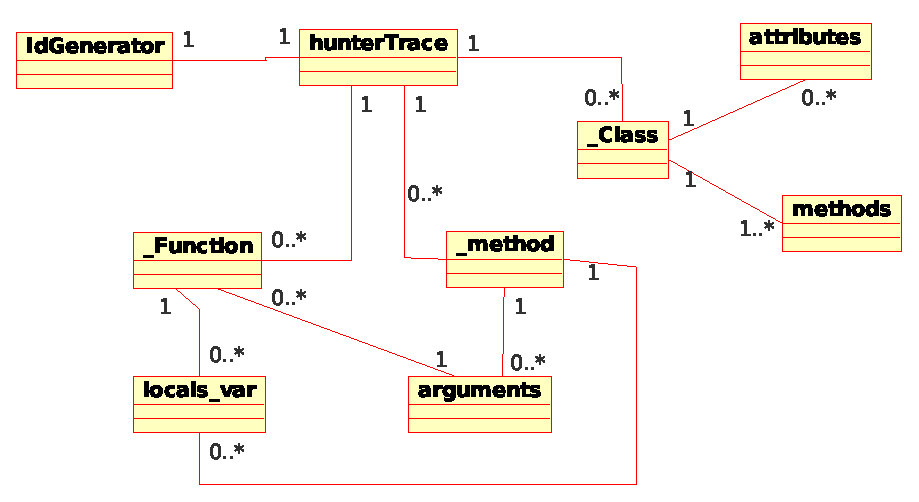
\includegraphics[scale=1]{images/class_diagram.eps}
	\caption{Diseño del capturador de huella}
\end{figure}

\pagebreak

\begin{thebibliography}{2}
\bibitem{inspect2} Module of Python: http://lfw.org/python/inspect.py
\bibitem{bytecode} Bytecode of Python: http://docs.python.org/lib/bytecodes.html
\end{thebibliography}
\end{document}